\documentclass[12pt,spanish]{article}
\usepackage[spanish]{babel}
\usepackage{graphicx}
\usepackage{multirow}
\usepackage[hidelinks]{hyperref}
\usepackage{caption}
\usepackage{multirow}
\usepackage{multicol}
\usepackage[outputdir=build]{minted}
\usepackage{float}
\usepackage{array}
\graphicspath{ {../img/} {../../LaTeX/img/} {/home/csp98/latex/img/}}
\selectlanguage{spanish}
\usepackage[utf8]{inputenc}
\usepackage{graphicx}
\usepackage[a4paper,left=3cm,right=2cm,top=2.5cm,bottom=2.5cm]{geometry}
\newtheorem{ppio}{Principio }
\makeindex

\begin{document}
\begin{titlepage}

\newlength{\centeroffset}
\setlength{\centeroffset}{-0.5\oddsidemargin}
\addtolength{\centeroffset}{0.5\evensidemargin}
\thispagestyle{empty}

\noindent\hspace*{\centeroffset}
\begin{minipage}{\textwidth}

\centering
\includegraphics[width=0.9\textwidth]{logo_ugr.jpg}\\[1.4cm]

\textsc{ \Large Algorítmica\\[0.2cm]}
\textsc{GRADO EN INGENIERÍA INFORMÁTICA}\\[1cm]

{\Huge\bfseries Ejercicio de clase\\}
\noindent\rule[-1ex]{\textwidth}{3pt}\\[3.5ex]
{\large\bfseries Búsqueda ternaria}
\end{minipage}

\vspace{1.5cm}
\noindent\hspace*{\centeroffset}
\begin{minipage}{\textwidth}
\centering

\textbf{Autores}\\ {Carlos Sánchez Páez}\\[2.5ex]
\includegraphics[width=0.3\textwidth]{etsiit_logo.png}\\[0.1cm]
\vspace{1.5cm}
\includegraphics[width=0.5\textwidth]{decsai.jpg}\\[0.1cm]
\vspace{1cm}
\textsc{Escuela Técnica Superior de Ingenierías Informática y de Telecomunicación}\\
\vspace{1cm}
\textsc{Curso 2017-2018}
\end{minipage}
\end{titlepage}
\tableofcontents
\thispagestyle{empty}
\listoftables
\listoffigures
\newpage
\setcounter{page}{1}

\section{Enunciado}
\large{Realizar un estudio empírico para determinar si es preferible utilizar la búsqueda binaria o la búsqueda ternaria comentada en clase (ambos algoritmos son de orden logarítmico, pero sus constantes ocultas son diferentes).}

\section{Resolución}

\subsection{Metodología}
Para resolver el ejercicio, ejecutaremos 25 veces cada código con tamaños de problema ascendentes mediante un \textcolor{blue!50}{\hyperref[script]{script}}.
Después, estudiaremos empíricamente su eficiencia y hallaremos el valor de sus constantes ocultas (eficiencia híbrida). Dentro del código fuente, cada algoritmo se ejecuta 1000 veces y se calcula el tiempo medio. Éste procedimiento se realiza ya que los tiempos son tan pequeños que cualquier mínima variación en la carga del sistema causada por otro proceso causa un gran efecto en el tiempo de ejecución, resultando en un gran pico en la representación gráfica. Igualmente, como los tiempos son tan pequeños, he tenido que utilizar el reloj que proporciona más precisión (\emph{high resolution clock}, de la biblioteca \textit{chrono}).

\begin{table}[H]
\centering
\begin{tabular}{|c|c|c|c|}
\hline
\textbf{Algoritmo} & \textbf{Tamaño inicial} & \textbf{Tamaño final} & \textbf{Incremento}\\
\hline
Búsqueda Binaria & & &\\
& 50.000.000  & 530.000.000 & 20.000.000\\
Búsqueda Ternaria & & &\\
\hline
\end{tabular}
\caption{Tamaños para la ejecución}
\end{table}

\subsection{Resultados obtenidos}
\begin{table}[H]
\centering
\begin{tabular}{|c|c|c|}
\hline
\textbf{Tamaño del problema} & \textbf{Búsqueda Binaria} & \textbf{Búsqueda Ternaria}\\
\hline
50.000.000 & 1.02815$\cdot 10^{-7}$ & \textcolor{green}{9.7679$\cdot 10^{-8}$}\\
\hline
70.000.000 & \textcolor{green}{9.9185$\cdot 10^{-8}$} & 1.02817$\cdot 10^{-7}$\\
\hline
90.000.000 & 1.87658$\cdot 10^{-7}$ & \textcolor{green}{9.4667$\cdot 10^{-8}$}\\
\hline
110.000.000 & \textcolor{green}{9.7568$\cdot 10^{-8}$} & 9.9846$\cdot 10^{-8}$\\
\hline
130.000.000 & 1.11688$\cdot 10^{-7}$ & \textcolor{green}{1.0234$\cdot 10^{-7}$}\\
\hline
150.000.000 & \textcolor{green}{1.09648$\cdot 10^{-7}$} & 1.25571$\cdot 10^{-7}$\\
\hline
170.000.000 & \textcolor{green}{9.5796$\cdot 10^{-8}$} & 1.01072$\cdot 10^{-7}$\\
\hline
190.000.000 & \textcolor{green}{1.1167$\cdot 10^{-7}$} & 1.23716$\cdot 10^{-7}$\\
\hline
210.000.000 & 1.08572$\cdot 10^{-7}$ & \textcolor{green}{1.04633$\cdot 10^{-7}$}\\
\hline
230.000.000 & \textcolor{green}{9.6589$\cdot 10^{-8}$} & 1.33206$\cdot 10^{-7}$\\
\hline
250.000.000 & \textcolor{green}{1.10112$\cdot 10^{-7}$} & 1.63717$\cdot 10^{-7}$\\
\hline
270.000.000 & 1.08413$\cdot 10^{-7}$ & \textcolor{green}{1.04575$\cdot 10^{-7}$}\\
\hline
290.000.000 & \textcolor{green}{1.12937$\cdot 10^{-7}$} & 1.50177$\cdot 10^{-7}$\\
\hline
310.000.000 & 1.11755$\cdot 10^{-7}$ & \textcolor{green}{1.10322$\cdot 10^{-7}$}\\
\hline
330.000.000 & 1.07642$\cdot 10^{-7}$ & \textcolor{green}{1.0309$\cdot 10^{-7}$}\\
\hline
350.000.000 & \textcolor{green}{1.07934$\cdot 10^{-7}$} & 1.11627$\cdot 10^{-7}$\\
\hline
370.000.000 & \textcolor{green}{1.04718$\cdot 10^{-7}$} & 1.09216$\cdot 10^{-7}$\\
\hline
390.000.000 & \textcolor{green}{1.04261$\cdot 10^{-7}$} & 1.23385$\cdot 10^{-7}$\\
\hline
410.000.000 & 1.7052$\cdot 10^{-7}$ & \textcolor{green}{1.02349$\cdot 10^{-7}$}\\
\hline
430.000.000 & 1.20473$\cdot 10^{-7}$ & \textcolor{green}{1.15399$\cdot 10^{-7}$}\\
\hline
450.000.000 & 1.21743$\cdot 10^{-7}$ & \textcolor{green}{1.07027$\cdot 10^{-7}$}\\
\hline
470.000.000 & 1.24807$\cdot 10^{-7}$ & \textcolor{green}{1.16637$\cdot 10^{-7}$}\\
\hline
490.000.000 & 1.45116$\cdot 10^{-7}$ & \textcolor{green}{1.1538$\cdot 10^{-7}$}\\
\hline
510.000.000 & \textcolor{green}{1.09658$\cdot 10^{-7}$} & 1.61301$\cdot 10^{-7}$\\
\hline
530.000.000 & 1.19847$\cdot 10^{-7}$ & \textcolor{green}{1.098$\cdot 10^{-7}$}\\
\hline
\hline
\textbf{Media} & \textcolor{green}{1,144$\cdot 10^{-7}$} & 1,507$\cdot 10^{-7}$\\
\hline
\end{tabular}
\caption{Tiempos obtenidos (seg)}
\end{table}

\subsection{Cálculo de la constante oculta}
Realizamos una regresión mediante \emph{gnuplot} para averiguar la constante:
\begin{table}[H]
\begin{tabular}{|c|c|c|}
\hline
\textbf{Algoritmo} & \textbf{Valor de la constante oculta} & \textbf{Porcentaje de error}\\
\hline
Búsqueda Binaria & 6.00559$\cdot 10^{-9}$ & 3.729\% \\
\hline
Búsqueda Ternaria & 5.98818$\cdot 10^{-9}$ & 3.074\%\\
\hline
\end{tabular}
\caption{Bondad del ajuste}
\end{table}
\newpage
\subsection{Gráficas}
Para apreciar mejor la curvatura de la representación, los ejes están expresados en escala logarítmica.
\begin{figure}[H]
\centering
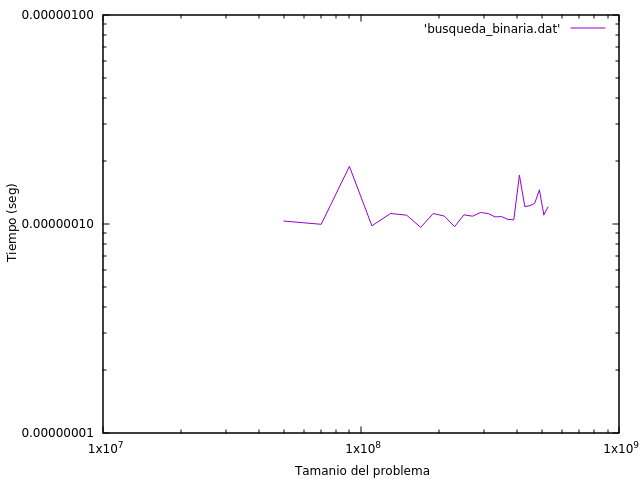
\includegraphics[scale=0.75]{empirica_binaria.png}
\caption{Eficiencia empírica. Búsqueda binaria}
\end{figure}

\begin{figure}[H]
\centering
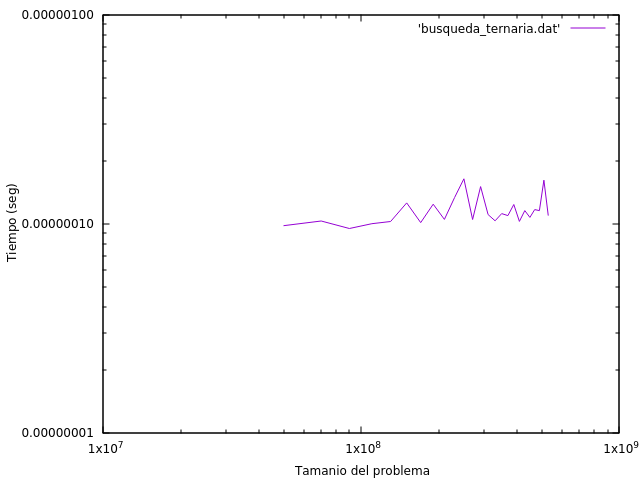
\includegraphics[scale=0.75]{empirica_ternaria.png}
\caption{Eficiencia empírica. Búsqueda ternaria}
\end{figure}

\begin{figure}[H]
\centering
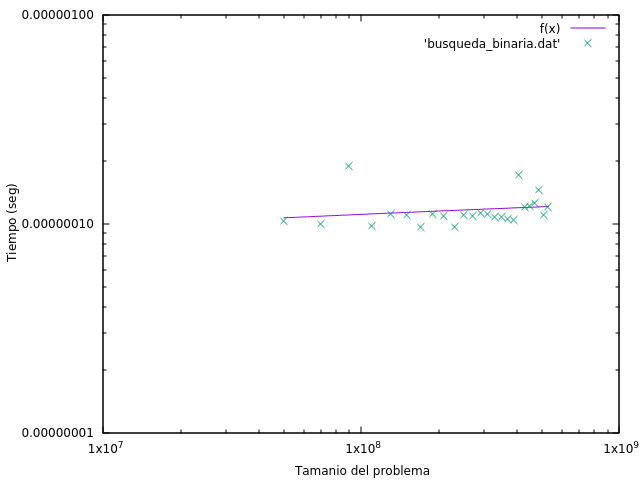
\includegraphics[scale=0.75]{hibrida_binaria.png}
\caption{Eficiencia híbrida. Búsqueda binaria}
\end{figure}

\begin{figure}[H]
\centering
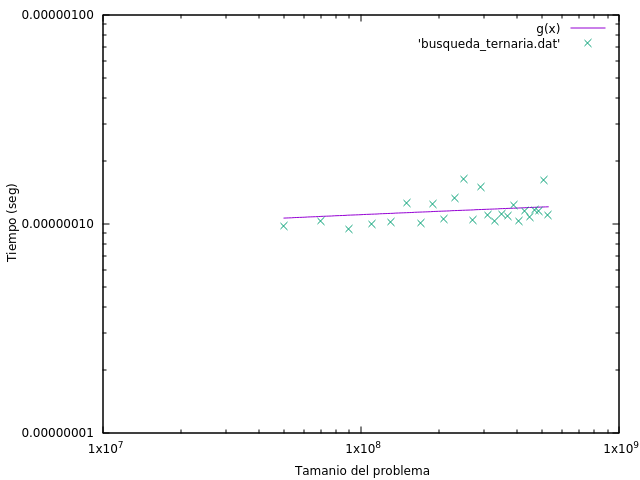
\includegraphics[scale=0.75]{hibrida_ternaria.png}
\caption{Eficiencia híbrida. Búsqueda ternaria}
\end{figure}

\newpage
\subsection{Conclusiones}
Tanto la búsqueda binaria como la ternaria tienen el mismo orden de eficiencia teórica ($O(\log n)$). Por tanto, la diferencia radicará en sus constantes ocultas. \\
Según la regresión realizada, la búsqueda ternaria tiene una constante oculta ligeramente menor a la binaria ($2 \cdot 10^{-11}$) Sin embargo, vemos como el ajuste de la binaria es peor (el porcentaje de error es un $0.7\%$ más). Si nos vamos a los tiempos empíricos, podemos confirmar que la búsqueda ternaria \textbf{no es más rápida} que la binaria, por lo que el nuevo algoritmo no nos proporciona ninguna mejora con respecto al tradicional.
\newpage
\subsection{Anexo:Algoritmos desarrollados}

\subsubsection{Búsqueda binaria}

\inputminted[linenos, fontsize=\footnotesize]{c++}{busqueda_binaria.cpp}

\newpage
\subsubsection{Búsqueda ternaria}

\inputminted[linenos, fontsize=\footnotesize]{c++}{busqueda_ternaria.cpp}


\subsubsection{Script para múltiples ejecuciones}
\label{script}

\inputminted[linenos, fontsize=\footnotesize]{bash}{individual.sh}

\subsubsection{Script de \emph{gnuplot}}

\inputminted[linenos, fontsize=\footnotesize]{bash}{gnuplot.sh}

\subsubsection{Script automatizado}

\inputminted[linenos, fontsize=\footnotesize]{bash}{all.sh}

\end{document}
